%=============================================================================
% Thesis Template in LaTex
%
% File:  06-Diskussion.tex -- Diskussion
% Author(s): Cyrano Golliez <golliezc@student.ethz.ch>
%
% Creation:  27 Jan 2014
% Time-stamp: <Tue 2013-08-13 20:14 juergen>
%
% Copyright (c) 2014 Infrastructure Management Group (IMG)
%               http://ibi.ethz.ch
%
% More information on LaTeX: http://www.latex-project.org/
%=============================================================================

\chapter{Diskussion}
\label{chap:Diskussion}

In diesem Kapitel wird die in Kapitel \ref{chap:Resultate} als optimal erachtete Lösung untersucht. Einerseits werden die Parameterauswahlen 1 bis 4 mit dem Grundzustand verglichen und andererseits werden die einzelnen Kostenstrukturen der verschiedenen Parameterauswahlen untersucht. Dies geschieht, um die als optimal erachtete Variante auf ihre Belastbarkeit zu prüfen.

\paragraph{Grundzustand}

Gemäss dem Risikovergleich in Kapitel \ref{chap:Resultate} ist im Grundzustand die bestmögliche Variante für die Zukunft von Uster die Variante 2.  
Bei näherer Betrachtung der in Abbildung \ref{img:KostenZ0} dargestellten Reisezeitkosten und Wartungskosten der Varianten wird deutlich, dass die Kosten die in der Variante 1 aufgrund der verlängerten Wartezeit entstehen, die Mehrkosten der Variante 2 infolge Bau und Wartung in einen Zeitraum von 40 Jahren um ein Vielfaches übersteigen. Die Mehrkosten, die bei der Ausführung der Variante 2 infolge höherer Bau- und Wartungskosten entstehen, betragen 1'238'600 CHF. Die Mehrkosten, die bei der Variante 1 aufgrund der höheren Reisezeitkosten entstehen betragen 38'984'439 CHF. 

Durch diesen Vergleich wird deutlich, dass sich die Variante 1, welche die Option \flqq nichts zu verändern\frqq darstellt, über den betrachteten Zeitraum von 40 Jahren nicht lohnen wird. Die Mehrkosten, die den Nutzern des Bahnübergangs und somit auch indirekt der Stadt Uster infolge der verlängerten Wartezeit entstehen, übersteigen die erforderlichen Investitionskosten für den Bau der Velounterführung um ein Vielfaches. Im Fall der Variante 3 trifft dies nicht zu, weshalb sich ein solches Investment unter den Annahmen des Grundzustandes nicht lohnt.

\begin{figure}[h!]
  \centering
  \subfloat[][]{\label{img:}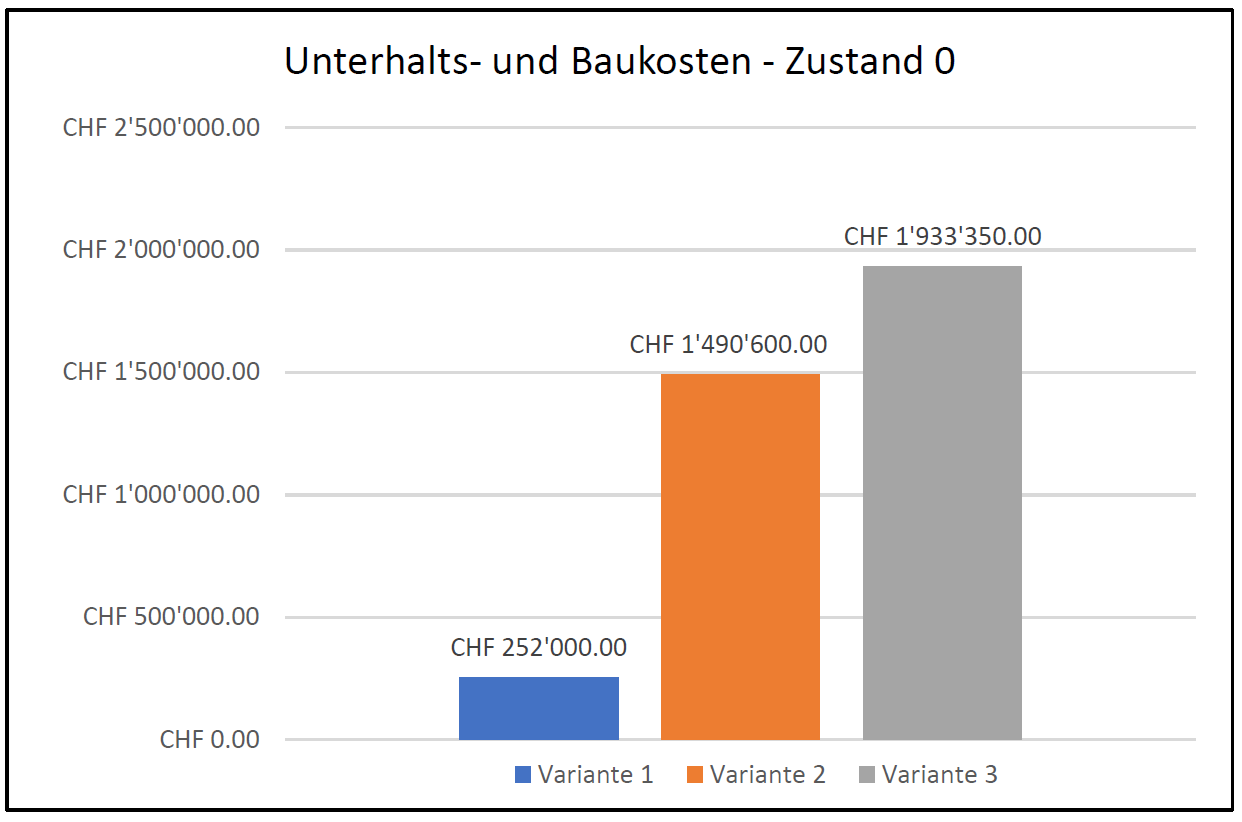
\includegraphics[width=.5\textwidth]{./figures/f-06-01-Unterhaltskosten-Z0}}
  \hfill
  \subfloat[][]{\label{img:}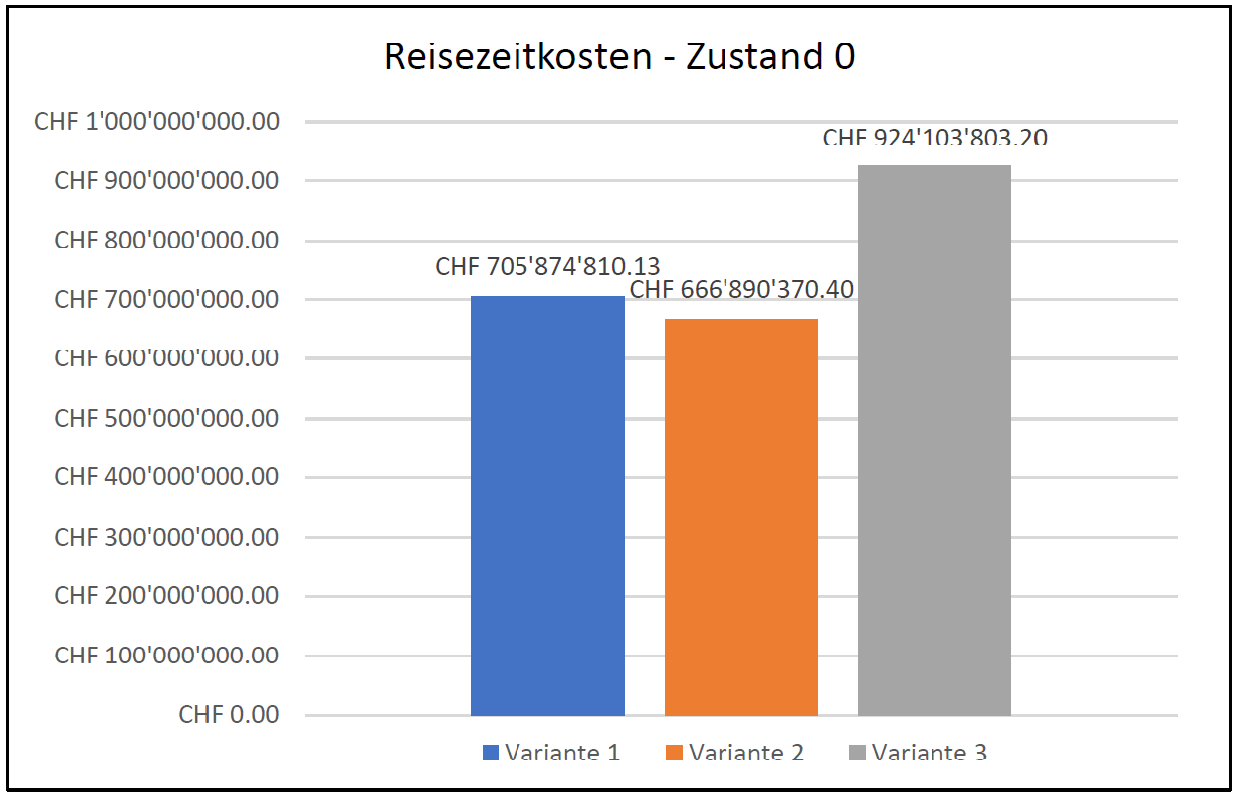
\includegraphics[width=.5\textwidth]{./figures/f-06-02-Reisezeitkosten-Z0}}
\caption[Kostenvergleich Grundzustand]{Kostenvergleich im Grundzustand}
  \label{img:KostenZ0}
\end{figure}

\begin{IMleftrightskip}
Die Kosten wurden analog der in Abschnitt \ref{subsec:BerechnungRisiken} erläuterten Risikoberechnung ermittelt. Dies gilt für alle weiteren erwähnten Kostenstrukturen.
\end{IMleftrightskip}

Demnach lohnt sich der Bau der Variante 2 für die Stadt Uster bei einer Betrachtung der Gesamtkosten über 40 Jahre. Das minimierte Risiko rechtfertigt die höheren Investitionskosten zu Beginn des untersuchten Zeitraums. 

\paragraph{Parameterauswahl 1: Veränderung E-Auto Anteil}

Gemäss Kapitel \ref{chap:Resultate} ist auch in der Parameterauswahl 1 die Variante 2 die optimale Lösung. Somit hat die Veränderung des E-Auto Anteiles keinen Einfluss auf die Wahl der optimalen Variante. \\
Infolge des Vergleichs des Grundzustandes und der Parameterauswahl 1 ist ersichtlich, dass das Risiko der Variante 1 um 0.023\%, das Risiko der Varianten 2 um 0.024\% und das Risiko der Variante 3 um 0.017\% gegenüber dem jeweiligen Risiko im Grundzustand ansteigt. Diese Abweichungen wären, um den Effekt der die Veränderung des E-Auto Anteiles auf optimale Lösung hat, im Rahmen einer Hauptstudie zu untersuchen.

Bei der näheren Betrachtung der Umweltkosten wird ersichtlich, dass die Umweltkosten für alle 3 Varianten jeweils um einen Betrag von 163'555 CHF ansteigen. Eine konservative Prognose des E-Auto Anteil hat somit keinen Einfluss auf die Wahl der optimalen Variante. Demnach müsste die Variante 2 auch in einer Zukunft in der der Verbrennungsmotor weiterhin eine massgebende Rolle spielen wird, die als optimal zu erachtende Variante sein, um die Verkehrssituation am Bahnübergang nachhaltig zu verbessern.


\paragraph{Parameterauswahl 2: Veränderung der Unfallwahrscheinlichkeit} 

Wie im Kapitel \ref{chap:Resultate} dargestellt, hat die Veränderung der Unfallwahrscheinlichkeit keinen Einfluss auf die Wahl der optimalen Variante. Bei näherer Betrachtung der Unfallkosten, sieht man, dass sich die Veränderung der Unfallwahrscheinlichkeit deutlich auf die anfallenden Unfallkosten auswirkt. 

Die Abbildung \ref{img:UnfallVer.Z0-2} zeigt den Unfallkostenvergleich des Grundzustandes und der Parameterauswahl 2. Die Unfallkosten aller Varianten im Grundzustand betragen 451'469 CHF. In der Parameterauswahl 2 betragen die Unfallkosten der Variante 2 547'384 CHF und die Unfallkosten der Variante 3 321'649 CHF. Für die Variante 2 entspricht das einer Veränderung von 21.25\% und für die Variante 3 einer Abnahme von 28.75\%. 

\begin{figure}[h!]
	\centering
	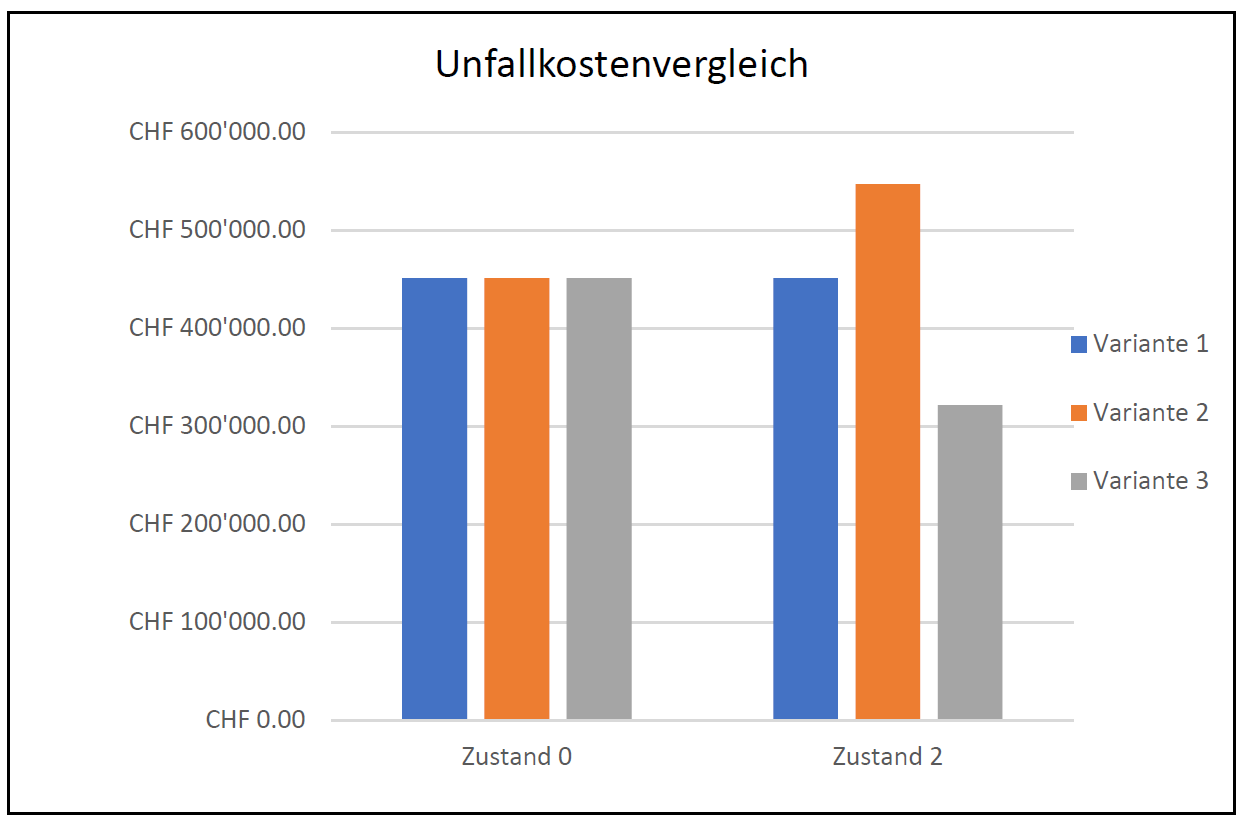
\includegraphics[width=.5\textwidth]{figures/f-06-03-Unfallkostenvergleich-Z0-Z2}
	\caption[Unfallkostenvergleich: Grundzustand und Parameterauswahl 2]{Unfallkostenvergleich des Grundzustandes und der Parameterauswahl 2}
	\label{img:UnfallVer.Z0-2}
\end{figure}

Betrachtet man hingegen die Veränderung der Risiken der Variante vom Grundzustand zur Parameterauswahl 2, so beträgt die Veränderung für die Variante 1 +0.01\% und für die Variante 3 -0.01\%. 
Somit ist die Variante 2 auch mit erhöhter Unfallgefahr die optimale Variante für die zukünftige Situation am Bahnübergang Brunnenstrasse. 
 

\paragraph{Parameterauswahl 3: Veränderung der Eintrittswahrscheinlichkeit} 

Die Veränderung der Eintrittswahrscheinlichkeit, wie in Abschnitt \ref{subsec:Sensitivitätsanalyse} dargestellt, hat keinen Einfluss auf die Wahl der optimalen Variante. Jedoch ist die folgende Darstellung \ref{img:SzeVer-Z0} der Risiken der einzelnen Szenarien, insofern interessant, dass es den Effekt verdeutlicht, den die Wahl der Eintrittswahrscheinlichkeit auf die Verteilung der Risiken hat. So können mit der Gewichtung der möglichen zukünftigen Ereignisse, sprich den Prognosen der möglichen Zukunft, die berechneten Risiken beeinflusst werden. 

\begin{figure}[h!]
	\centering
	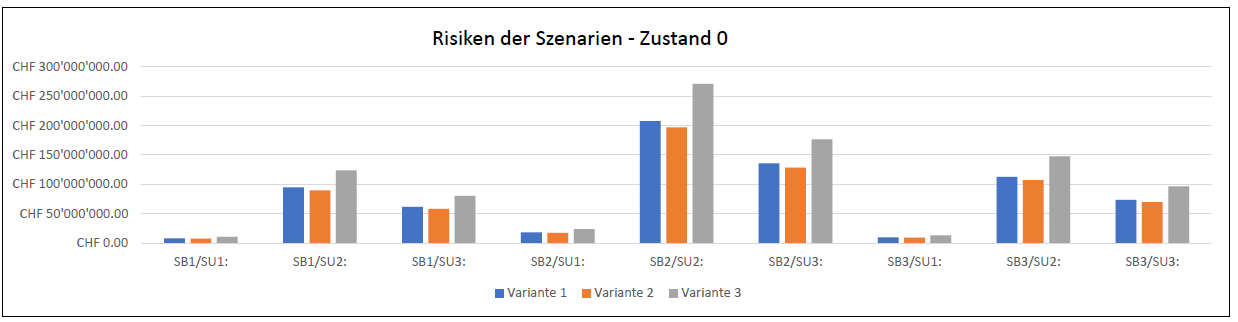
\includegraphics[width=\textwidth]{figures/f-06-04-RisikenSzenarienZ0}
	\caption[Szenarienvergleich im Grundzustand]{Vergleich der Risiken der Szenarien im Grundzustand}
	\label{img:SzeVer-Z0}
\end{figure} 

In der Parameterauswahl 3 wird der Schwerpunkt der Gewichtung der Szenarien so gelegt, dass diejenigen Szenarien mehr Gewicht erhalten, welche die höchsten Wachstumsprognosen voraussagen und demnach das grösste Verkehrsaufkommen implizieren. Der Effekt einer solchen Verschiebung auf die Szenarien wird in der nachfolgenden Abbildung \ref{img:SzeVer-Z3} dargestellt. 

\begin{figure}[h!]
	\centering
	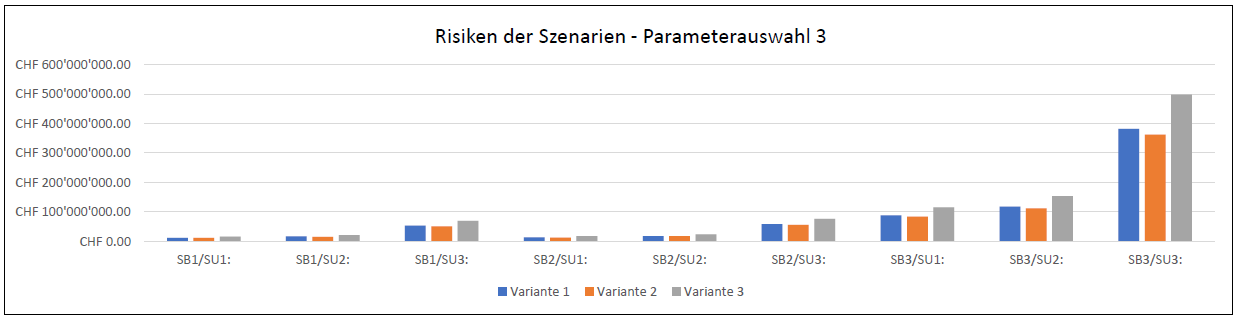
\includegraphics[width=\textwidth]{figures/f-06-05-RisikenSzenarienZ3}
	\caption[Szenarienvergleich Parameterauswahl 3]{Vergleich der Risiken der Szenarien für die Parameterauswahl 3}
	\label{img:SzeVer-Z3}
\end{figure} 

Auf die Wahl der optimalen Variante hat diese Veränderung keinen Einfluss, da die Risiken der Varianten jeweils um 5.5\% im Vergleich zum Grundzustand steigen. Erst bei der Betrachtung der Nachkommastellen, lässt sich eine gewisse Unterscheidung feststellen. So beträgt die Veränderung des Risiko der Variante 1 vom Grundzustand zur Parameterauswahl 3 5.530\%, die Veränderung des Risiko der Variante 2 beträgt 5.518\% und die Veränderung des Risikos der Variante 3 5.525\%. Aus diesen geringfügigen Abweichungen einen Rückschluss auf die im Rahmen der Parameterauswahl 3 veränderten Eigenschaften der Risikoberechnung zu machen, war im Rahmen dieser Projektarbeit nicht möglich und wäre im Rahmen einer Hauptstudie weiter zu untersuchen.


\paragraph{Parameterauswahl 4: Veränderung der Reisezeit} 

Wie in Kapitel \ref{chap:Resultate} ermittelt, ist in der Parameterauswahl 4 das Risiko der Variante 3 um 38'095 CHF kleiner als das Risiko der Variante 2. Das Risiko der Variante 1 bleibt unverändert und aufgrund dessen ist die optimale Variante für die Parameterauswahl 4 die Variante 3. \\
Die getroffenen Annahme über die Wartezeit der Variante 3 für die Parameterauswahl 4 vernachlässigt das Ampelsystem und berücksichtigt demnach nicht, eine verlängerte Reisezeit aufgrund der Rotlichtzyklen des Ampelsystems. 

Den Einfluss dieser Veränderung sieht man verdeutlicht bei den Reisezeitkosten. So nehmen die Reisezeitkosten der Variante 3 vom Grundzustand zur Parameterauswahl 4 um 257'694'277 CHF ab, wie in Abbildung \ref{img:ReisezeitkostenZ0-Z4} ersichtlich ist. Die Reisezeitkosten der Varianten 1 und 2 bleiben für die Parameterauswahl 4 unverändert, da ihre gemäss Abschnitt \ref{sec:Kostenstruktur} definierten Parameter der Kostenberechnung nicht verändert werden. So betragen die Reisezeitkostend der Variante 1 sowohl im Grundzustand als auch für die Parameterauswahl 4 705'874'810 CHF und die Reisezeitkosten der Variante 2 666'890'370 CHF.


\begin{figure}[h!]
	\centering
	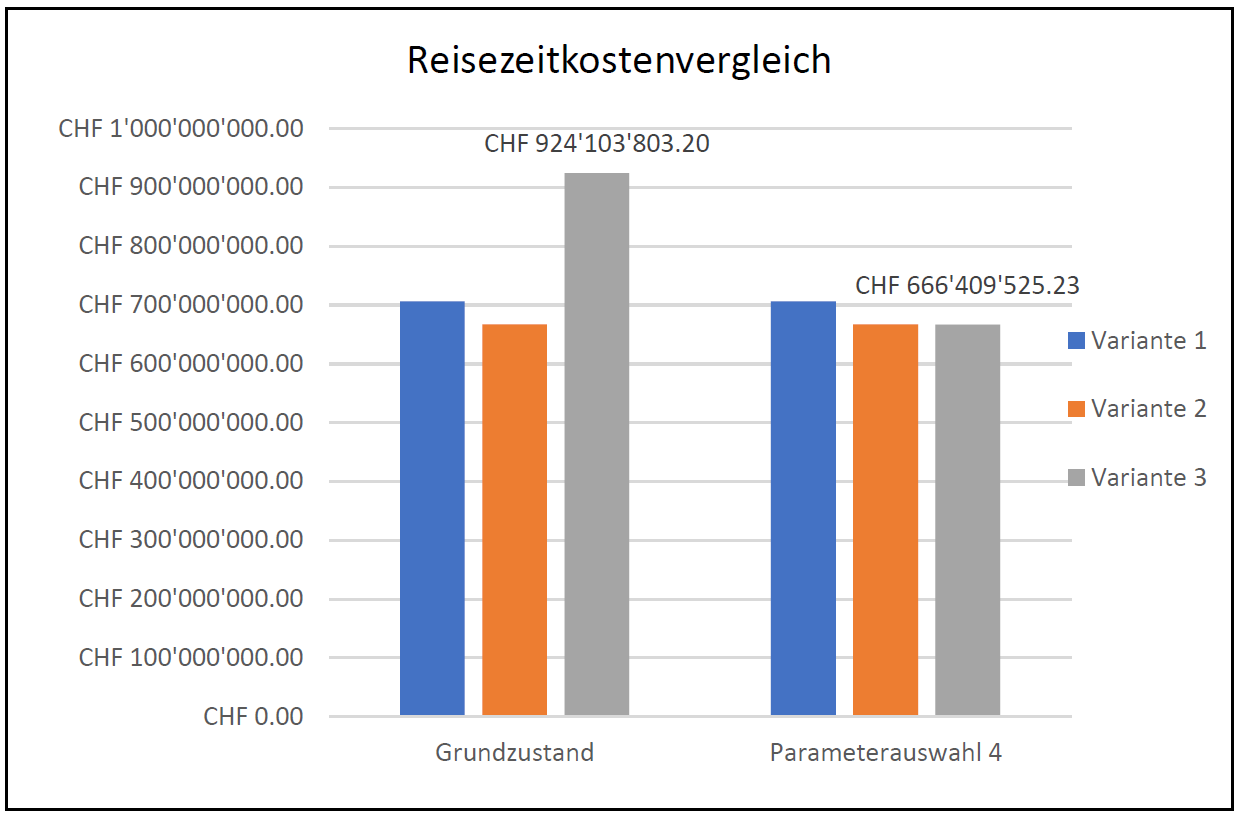
\includegraphics[width=.45\textwidth]{figures/f-06-06-ReisezeitVergleichZ0-Z4}
	\caption[Reisezeitkostenvergleich Grundzustand und Parameterauswahl 4]{Reisezeitkostenvergleich Grundzustand und Parameterauswahl 4}
	\label{img:ReisezeitkostenZ0-Z4}
\end{figure} 

Bei näherer Betrachtung der Reisezeitkosten der Variante 2 und Variante 3 wird deutlich weshalb die Variante 3 für die Parameterauswahl 4 das geringste Risiko generiert. \\
In Abbildung \ref{img:ReisezeitkostenV2-V3-Z4} ist ersichtlich, dass die Reisezeitkosten der Variante 2 666'890'370 CHF betragen und die Reisezeitkosten der Variante 3 für die Parameterauswahl 4 nur noch 666'409'525 CHF. So nehmen die Reisezeitkosten der Variante 3 in der Parameterauswahl 4 um 27.89\% gegenüber dem Grundzustand ab. Das Risiko hingegen der Variante 3 für die Parameterauswahl 4 nimmt um 27.38\% gegenüber dem Risiko im Grundzustand ab.

\begin{figure}[h!]
	\centering
	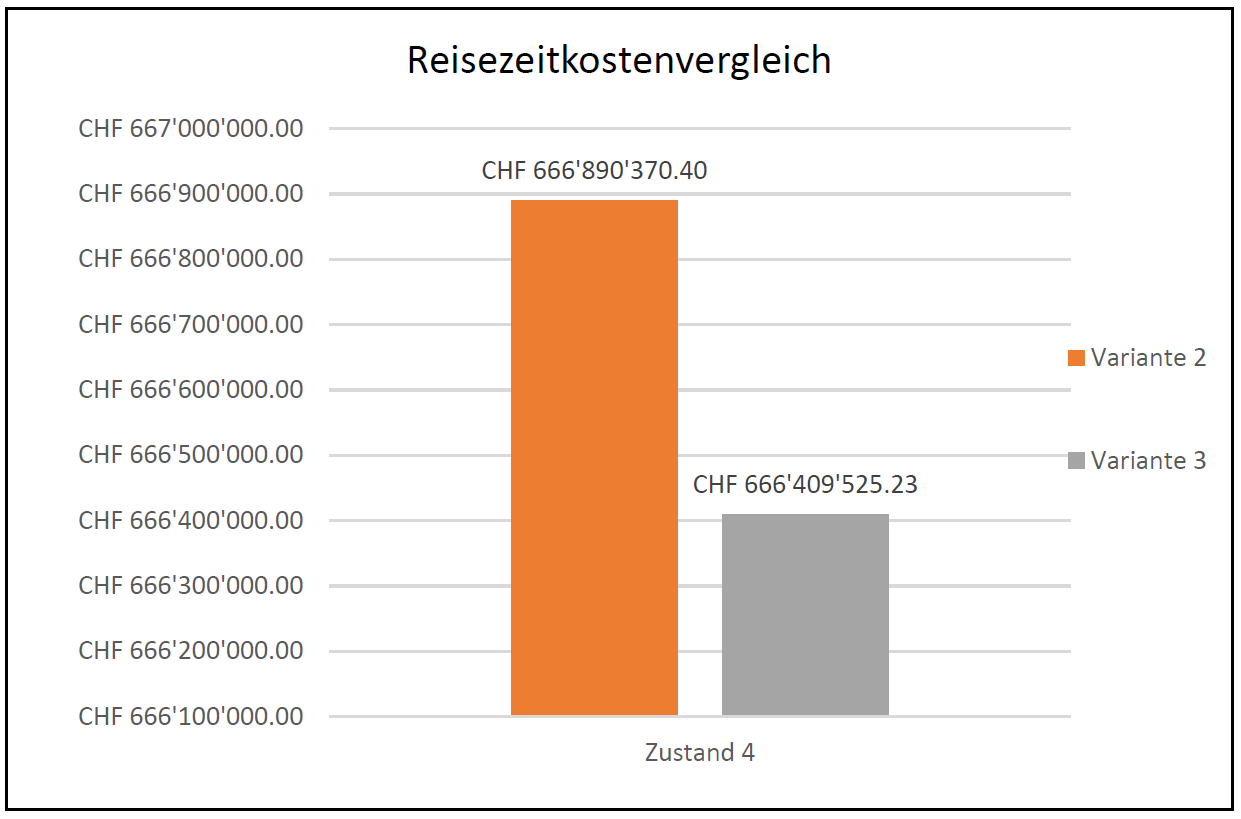
\includegraphics[width=.45\textwidth]{figures/f-06-07-ReisezeitVergleichV2_V3-Z0}
	\caption[Reisezeitkostenvergleich Variante 2 und 3 Parameterauswahl 4]{Reisezeitkostenvergleich Variante 2 und 3 für die Parameterauswahl 4}
	\label{img:ReisezeitkostenV2-V3-Z4}
\end{figure} 

Die Differenz der Reisezeitkosten der Varianten 2 und 3 beträgt 480'845 CHF, wobei die Differenz der Risiken der Varianten 2 und 3 in der Parameterauswahl 4 gemäss Kapitel \ref{chap:Resultate} 38'095 beträgt. So wird deutlich, dass einerseits die Reisezeit der entscheidende Faktor für die Risikoberechnung ist und andererseits, dass die im Rahmen der Optimierung des Bahnübergangs Brunnenstrasse notwendigen Entscheidungsprozesse von den Annahmen der zu erwartenden Reisezeiten abhängig sind.
Des weiteren ist ersichtlich, dass die Mehrkosten die beim Bau der Variante 3 im Vergleich zu Variante 2 entstehen, gemäss Abschnitt \ref{sec:Varianten} 347'750 CHF, von den grösseren Reisezeitkosten der Variante 2 kompensiert werden. Die verbleibende Differenz der Risiken von 38'095 CHF und die daraus folgende Wahl der Variante 3 als optimale Variante muss aufgrund dessen, dass die getroffenen Annahmen in der Parameterauswahl 4 nicht unbedingt der Wirklichkeit entsprechen, von einem kritischen Standpunkt aus betrachtet werden.

Meiner Meinung nach entspricht die getroffene Annahme, dass die Wartezeit der Variante 3 aufgrund der Einführung eines Ampelsystems nicht ansteigt, nicht der Realität. \\
So wird bei der Betrachtung der jetzigen Situation am Bahnübergang klar, dass sich die Wartezeit aufgrund von Rückstaus, bedingt durch die Verkehrsüberlastung der Innenstadt, zu Hauptverkehrszeiten deutlich verlängert. Infolge wird die Einführung eines Ampelsystems aufgrund der beengten Platzverhältnisse vor Ort zu, wie für den Grundzustand sowie für die Parameterauswahlen 1, 2 und 3 angenommen, einer erhöhten Wartezeit führen, was den Annahmen der Parameterauswahl 4 wiederspricht.

Die Wahl der Variante 3 zur optimalen Variante für die Parameterauswahl 4 hat auf den Entscheidungsprozess keine Einfluss. Nimmt man an, dass sich die Wartezeiten für alle 3 Varianten, aufgrund der Einführung einer neuen S-Bahn Linie gleichmässig erhöht, so lohnt sich das grössere Investment der Variante 3 nur bei einer Betrachtung der Situation über einen Zeitraum von vierzig Jahren. 

Die Variante 3 könnte sich für die Stadt Uster lohnen, da das eingeführte Ampelsystem eine Verschiebung des innerstädtischen Modalsplit zur Folge haben kann und dadurch der Veloverkehr gefördert wird, was sich wiederum in den Unfall- und Umweltbelastungskosten wiederspiegelt.

In dieser Diskussion werden die Mehrwerte der Variante 3, die aufgrund der erhöhten Sicherheit sowie des erhöhten Fahrkomfort entstehen, ausser Acht gelassen. Die Velounterführung der Variante 2 mit ihren 1.5 Meter lichten Breite hat im Vergleich zur Variante 3 mit über 2 Metern Durchfahrtsbreite, einen deutlich geringeren Fahrkomfort und dementsprechend auch ein erhöhtes Unfallrisiko. Somit kann für die Parameterauswahl 4, mit den mir zur Verfügung stehenden Mitteln nicht abschliessend geklärt werden, ob  Variante 3 die optimale Variante ist.
      

% ===========================================================================
% EOF
%

%%% Local Variables:
%%% mode: latex
%%% TeX-master: "../main"
%%% End:
